For clarity, add labels to the shaded quadrilateral: 
\begin{figure}[H]
\centering
\includegraphics[height=5cm,page=2]{quadrilateral-area-shaded}
\end{figure}
The area of the quadrilateral NESW is equal to half the product of its diagonals, NS and ES. If we denote by $h$ the vertical diagonal NS, or `height', and by $w$ the horizontal diagonal EW, or `width', the area is given by:
\begin{align*}
\frac{wh}{2}
 = 
\frac{\text{EW} \times \text{NS}}{2}
\end{align*}
where S is the intersection of the diagonals of the square ABCD (the center of the square), and N is the intersection of the diagonals of the rectangle CDPQ.

The height of the quadrilateral follows immediately from the ``Intercept Theorem''. The Intercept theorem states that Given two parallel lines AC and BD and some point S, the following ratios hold:
\begin{align*}
\frac{\text{SA}}{\text{SB}} 
  = \frac{\text{SC}}{\text{SD}} 
  = \frac{\text{AC}}{\text{BD}} 
\end{align*} 
\begin{figure}[H]
\centering
\includegraphics[height=6cm,page=6]{quadrilateral-area-shaded}
\end{figure}

Applying the Intercept Theorem to point D and the parallel lines NS and QB gives:
\begin{align*}
\frac{\text{DQ}}{\text{DN}} 
  = \frac{\text{DB}}{\text{DS}} 
  = \frac{\text{QB}}{\text{NS}} 
\end{align*}
and since $\text{DB}=2\text{DS}$ (the center of the square S cuts the diagonal DB in half) and $\text{QB}=b$ (as stated in the question), it follows that the height of the quadrilateral is
\begin{align*}
h = \text{NS} = \frac{b}{2}
\end{align*}
\begin{figure}[H]
\centering
\includegraphics[height=10cm,page=3]{quadrilateral-area-shaded}
\end{figure}
Next, we calculate the width of the quadrilateral. Let $w$ denote the length of EW and let $x$ denote the length of $\text{E}\text{E}^{\prime}$. Since the square has side length $a$, we have $x+w+x=a$ (see the figure), or $w=a-2x$. Thus, $w$ follows from $x$: it is easier to calculate $x$. 
\begin{figure}[H]
\centering
\includegraphics[height=10cm,page=4]{quadrilateral-area-shaded}
\end{figure} 

It is easier to calculate $x$ than $w$, because the existence of a square of side length $x$ allows us to change perspective. Earlier we found it quite straightforward to calculate the vertical distance $h$ by applying the Intercept theorem, because of the existence of two parallel lines intersecting an angle at known distances. Applying similar reasoning to $w$ leads us to consider triangle CSD and the parallel lines EW and DC (see figure below). Unfortunately, the distances needed to apply the Intercept theorem are not immediately known. By contrast, applying similar reasoning to $x$ gives several ways to apply the Intercept theorem. We could consider triangle DQC and the parallel lines $\text{E}\text{E}^{\prime}$ and DC. Or we could consider triangle CDQ and the parallel lines $\text{E}^{\prime\prime}\text{E}$ and CQ. 

\begin{figure}[H]
\centering
\includegraphics[height=10cm,page=8]{quadrilateral-area-shaded}
\end{figure} 

Consider triangle CDQ. Because CE is on the diagonal of square ABCD, it is a bisector of DCQ, and therefore it is the diagonal of square $\text{C}\text{E}^{\prime}\text{E}\text{E}^{\prime\prime}$. Thus, the lengths of $\text{C}\text{E}^{\prime\prime}$ and $\text{E}\text{E}^{\prime}$ are equal, implying that triangles CDQ and  $\text{E}^{\prime\prime}\text{D}\text{E}$ are similar. For two similar triangles, the ratio of their legs are equal, for instance:
\begin{align*}
\frac{\text{C}\text{D}}{\text{C}\text{Q}} 
= \frac{\text{E}^{\prime\prime}\text{D}}{\text{E}^{\prime\prime}\text{E}}  
\end{align*}
Focusing on triangle CDQ makes this clearer:
\begin{figure}[H]
\centering
\includegraphics[height=8cm,page=5]{quadrilateral-area-shaded}
\end{figure}
From $\text{CD}=a$, $\text{CQ}=a-b$ and   $\text{C}\text{E}^{\prime\prime}=\text{E}^{\prime\prime}\text{E}=\text{E}\text{E}^{\prime}=x$, we get $\text{E}^{\prime\prime}\text{D}=CD-\text{C}\text{E}^{\prime\prime}=a-x$. Substituting known lengths into the above relation yields an equation in $x$:
\begin{align*}
\frac{a}{a-b} = \frac{a-x}{x} 
\end{align*}
which may be solved for $x$ in terms of $a,b$, from which $w$ follows: 
\begin{align*}
x & = \frac{a(a-b)}{2a-b} \\
w & = a - 2x 
    = a - 2 \times \frac{a(a-b)}{2a-b} 
    = \frac{a(2a-b)-2a(a-b)}{2a-b}
    = \frac{ab}{2a-b}
\end{align*}
The area of the quadrilateral is then:
\begin{align*}
\frac{b}{2} \times \frac{ab}{2(2a-b)}
  = \frac{ab^2}{4(2a-b)}
\end{align*}
In the special case $a=6$ and $b=1$ (the values in the Chapter Invitational), the area is
\begin{align*}
\frac{ab^2}{4(2a-b)}
 = \dfrac{3}{22}~\text{units}^{2}
\end{align*}

\newpage 
In a solution provided in association with MathCounts, Prof. Po Shen Loh showed a different approach to calculate $w$, somewhat easier and faster. Consider the system of Cartesian coordinates centered at point A, with $x$-axis along AB and $y$-axis along AD. In this system, diagonal AC has equation $y=x$ (the $45^{\circ}$ line), while line DQ has equation
\begin{align*}
y = a - \frac{a-b}{a} x
\end{align*}
The intercept is obviously $a$ (the side length AD), while the slope is the vertical displacement, $-(a-b)$ (length of segment CQ, with a negative sign to mark the descent), divided by the horizontal displacement, $a$ (length of segment DC).
\begin{figure}[H]
\centering
\includegraphics[height=12cm,page=7]{quadrilateral-area-shaded}
\end{figure}
Half the width of the quadrilateral is then the $x$-coordinate of point E minus the $x$-coordinate of the center of the square. Thus,
\begin{align*}
w = 2\left(x_{\text{E}} - \frac{a}{2}\right)
\end{align*}

The value of $x_{\text{E}}$ is found by solving the system:
\begin{align*}
\begin{cases}
y ~= & x \\
y ~= & a - \dfrac{a-b}{a} x
\end{cases}
\end{align*}
which yields $w$ once again:
\begin{align*}
x_{\text{E}} = \frac{a^2}{2a-b}, 
  \quad
w = 2\left(x_{\text{E}} - \frac{a}{2}\right)
  = 2 \left(\frac{a^2}{2a-b}-\frac{a}{2}\right)
  = \frac{2a^2-a(2a-b)}{2a-b}
  = \frac{ab}{2a-b}
\end{align*}
